\documentclass[11pt, twocolumn]{article}
\usepackage{mathptmx} % Times New Roman
\usepackage{graphicx}
\graphicspath{{figures/}}
\usepackage{amsmath,amssymb}
\usepackage{hyperref}
\hypersetup{
    colorlinks=true,        % Enable colored links
    linkcolor=blue,         % Set the color for internal links (like sections, tables)
    filecolor=magenta,      % Color for file links
    urlcolor=cyan,          % Color for external URLs
    citecolor=red         % Color for citations
}
\usepackage{subfigure}
\usepackage{listings}
\lstset{
  language=Python,                % Language for syntax highlighting (e.g., Python, Matlab, C++)
  basicstyle=\ttfamily\footnotesize, % Code font size and style
  frame=single,                  % Adds a frame around the code
  breaklines=true,               % Line breaking
}
\usepackage{caption}
\usepackage{stfloats}
\usepackage{changepage}
\usepackage{setspace}
\setlength{\parskip}{1em} 
\usepackage{titling}
\setlength{\droptitle}{-7em}
\captionsetup{font=small, labelfont=bf, textfont=it, aboveskip=8pt, belowskip=2pt}
\hypersetup{colorlinks=true, urlcolor=blue, linkcolor=black, citecolor=red}
\setlength{\parindent}{0pt}

\usepackage[a4paper,top=2.5cm,bottom=2.5cm,left=2cm,right=2cm,marginparwidth=1.75cm]{geometry}

\begin{document}
\singlespacing
\title{\Large \textbf{3G3 Lab Report: Coding in Visual Cortex}}
\author{Shanzi(Monica) Ran\\
sr2021@cam.ac.uk}
\date{\small \today}
\maketitle

\section{Introduction}

Neural coding is a widely studied framework for sensory information processing, aiming to maximize the metabolic or informational efficiency of sensory representations \cite{willmore_2001_characterizing}. This report compares two coding strategies at the primary visual cortex (V1):

\begin{itemize}
\item Compact coding: A small population of neurons represents stimuli with frequent activation, reducing redundancy in visual representation \cite{olshausen_2004_sparse, field_1994_what}.
\item Sparse coding: Stimuli are represented by a small number of basis functions from a large set, producing a dispersed and sparse representation of sensory input \cite{olshausen_2004_sparse,field_1994_what}.
\end{itemize}

Through linear algebra simulations, this report explores these coding schemes using both natural and generated images, analyzing how image statistics influence the representation and performance of coding schemes.

\vspace{-1em}
\section{Results and Discussion}
\vspace{-1em}
\subsection{Datasets}
\vspace{-1em}
\begin{figure}[ht]
    \centering
    \subfigure[\textit{I1} (book scan)]{
        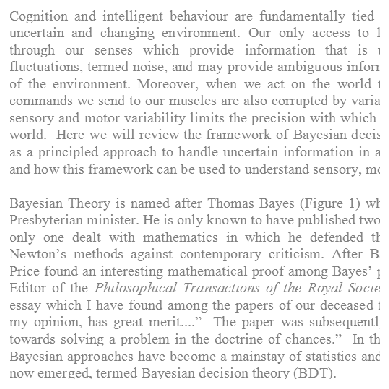
\includegraphics[width=0.2\textwidth]{1-1.png}
    }
    \subfigure[\textit{I2} (natural image)]{
        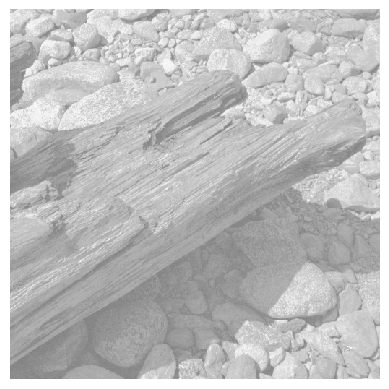
\includegraphics[width=0.2\textwidth]{1-2.png}
    }
    \subfigure[\textit{I2w} (whitened I2)]{
        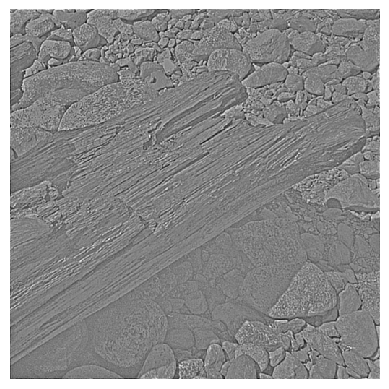
\includegraphics[width=0.2\textwidth]{1-3.png}
    }
    \subfigure[\textit{I3} (random white noise)]{
        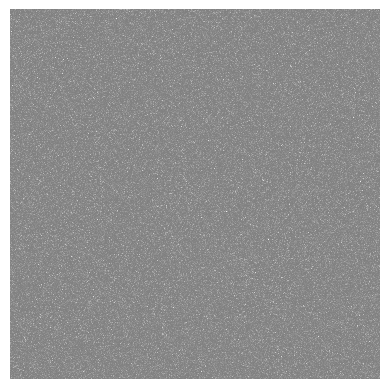
\includegraphics[width=0.2\textwidth]{1-4.png}
    }
    \caption{Examples of images from each of the categories}
    \label{fig:1}
\end{figure}

\textbf{A1} Natural images, such as scenes from the natural world \cite{zhu_2023_statistics}, exhibit high local pairwise correlation, resulting in a significantly smaller state space compared to randomly generated noise. The greyscale image sets used in this exercise (Fig~\ref{fig:1}) are categorized as follows: \textit{I1} consists of natural scenes, \textit{I2} contains book scans, and \textit{I3} comprises synthetic white noise images. Additionally, \textit{I2w} represents a whitened version of \textit{I2}, where whitening reduces redundancy by decorrelating adjacent pixels and normalizing variance. \textbf{EOA}

\subsection{Compact Coding}

\vspace{-1em}

\subsubsection{Dimension Reduction}\label{sec:dimreduction}

\vspace{-1em}

The dimension reducing compact coding algorithm employed in this exercise is Principal Components Analysis (PCA), which produces a hierarchy of eigenvectors of the covariance matrix according to the eigenvalues (variance). 
\textbf{A2} Using this hierarchy, it is observed in the exercise that 102 principal components (PC) capture 90\% of the variance in the semi-random book scan \textit{I1} that contains man-made features \cite{field_1994_what} \textbf{EOA}, \textbf{A4} 191 components are needed for \textit{I3}, reflecting its random nature and full state space \textbf{EOA}, and \textbf{A5} 16 components suffice for \textit{I2}, consistent with the high redundancy of natural images \textbf{EOA}. Nevertheless, these values all show a reduction from the original 256-dimensional space.

\subsubsection{Interpretation of Bases by PCA}
Due to statistical differences across image categories, the PCA basis functions for datasets \textit{I1}, \textit{I2}, and \textit{I3} will be analyzed separately in the following section.
\paragraph{PCA for \textit{I1}}


\vspace{-1em}
\textbf{A3} For book scan \textit{I1}, each PC captures distinct printing features and setting. For example, the basis function in Fig~\ref{fig:3} captures the spacing between words on the page. The density distribution of the spacing is also depicted in the filter shape. \textbf{EOA}
\begin{figure}[ht]
    \centering
    \subfigure[]{
        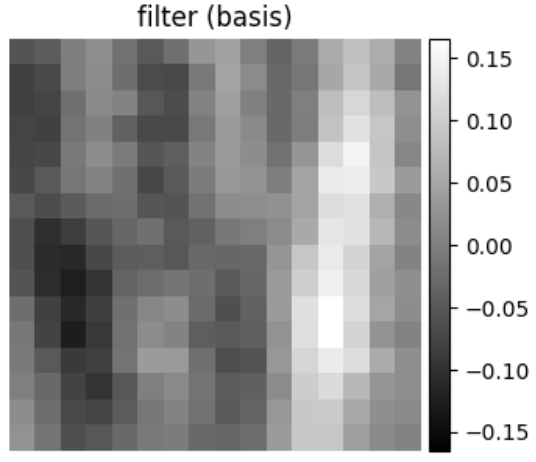
\includegraphics[width=0.155\textwidth]{3-3.png}
    }
    \subfigure[]{
        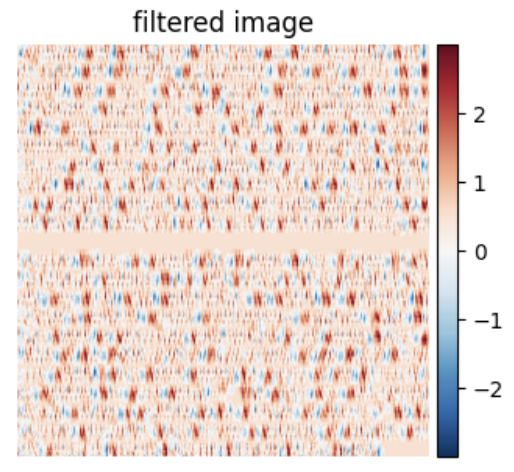
\includegraphics[width=0.145\textwidth]{3-1.png}
    }
    \subfigure[]{
        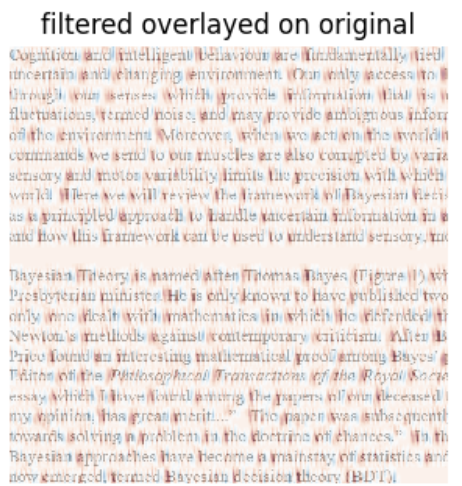
\includegraphics[width=0.13\textwidth]{3-2.png}
    }
    \caption{An example of basis function for book scan \textit{I1}: (a)basis filter, (b)filtered image, (c)filtered image overlayed on original image}
    \label{fig:3}
\end{figure}

\paragraph{PCA for \textit{I2}}

\textbf{A6} For natural image in \textit{I2}, PCA performs a feature extraction transformation similar to principal edge detection. It is also observed that the bases are ordered by increasing complexity, and the whole set of PCs is constructed by rotations of basis coordinates.\textbf{EOA}

\begin{figure}[ht]
    \centering
    \subfigure[]{
        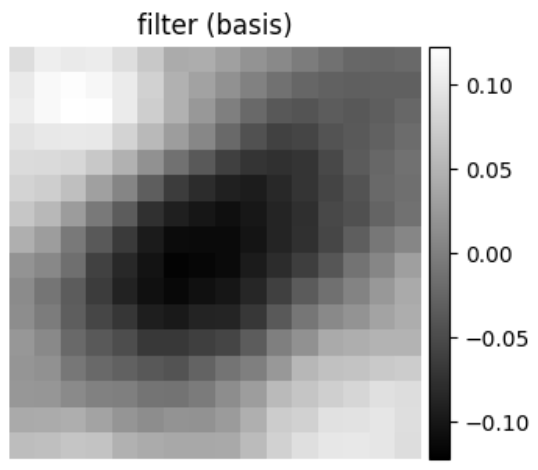
\includegraphics[width=0.15\textwidth]{5-1.png}
    }
    \subfigure[]{
        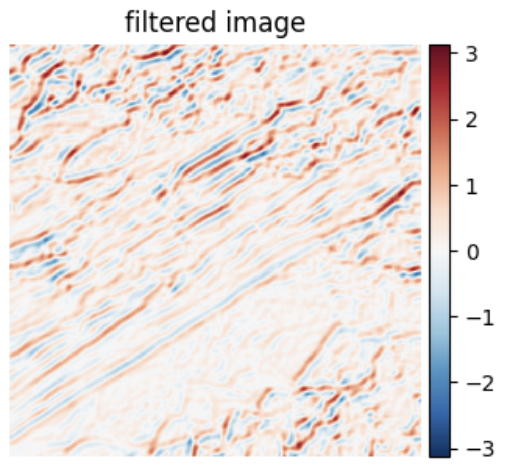
\includegraphics[width=0.14\textwidth]{5-2.png}
    }
    \subfigure[]{
        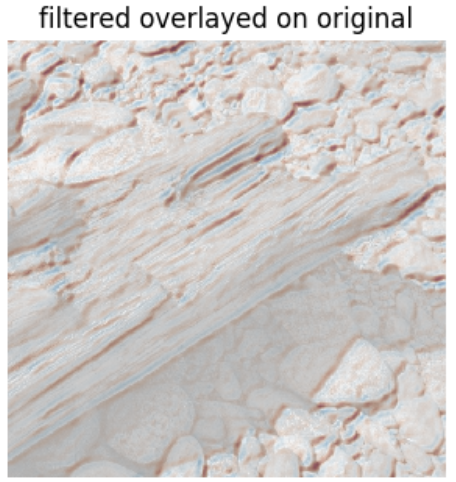
\includegraphics[width=0.12\textwidth]{5-3.png}
    }
    
    \subfigure[]{
        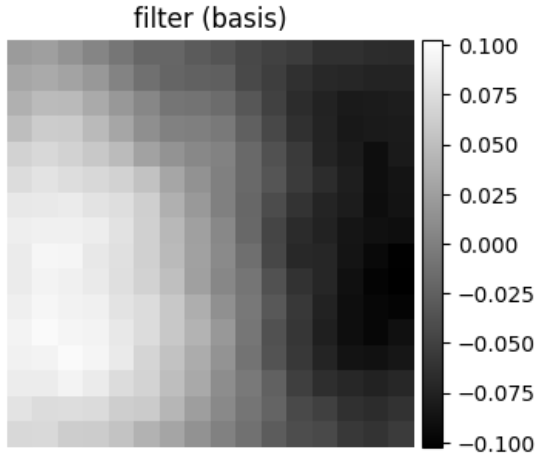
\includegraphics[width=0.15\textwidth]{5-4.png}
    }
    \subfigure[]{
        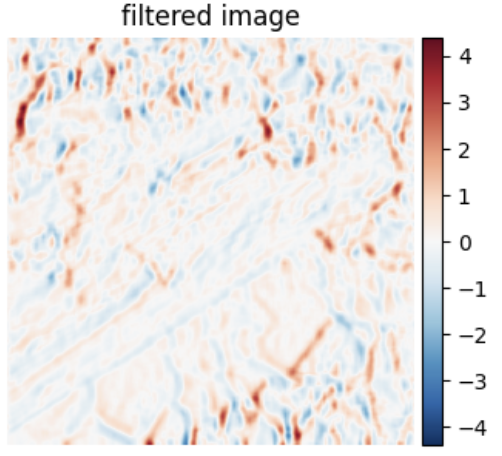
\includegraphics[width=0.14\textwidth]{5-5.png}
    }
    \subfigure[]{
        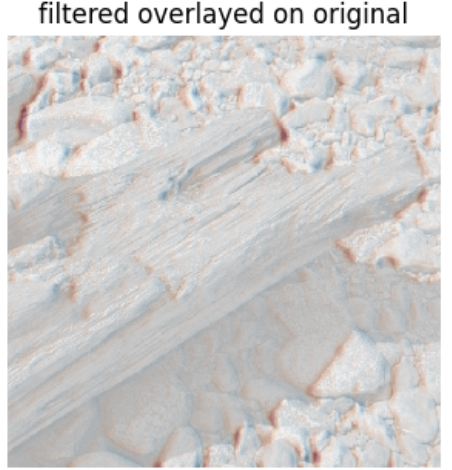
\includegraphics[width=0.12\textwidth]{5-6.png}
    }
    \caption{Two examples of basis functions for natural image \textit{I2}, where (a)(d) are basis filters, (b)(e) are filtered images, and (c)(f) are filtered image overlayed on original image. It can be observed that (a)(b)(c) depicts a filter detecting edge in diagonal direction, while (d)(e)(f) depicts another filter detecing edge concentrated in the corner orthogonal to the first filter.}
    \label{fig:5}
\end{figure}

\textbf{A5} For example, two of the PC bases shown in Fig~\ref{fig:5} demonstrate different edge detecting directions, which highlights edges aligned to the filter negative weight areas accordingly. 
This result aligns with expectation as edges representing first-order derivative change in the observed direction are indeed fundamental components constructing an image. It may also be noted that the filter eliminates redundancy by reducing contrast in areas not aligned to the filer. \textbf{EOA}

\begin{figure}[ht]
    \centering
    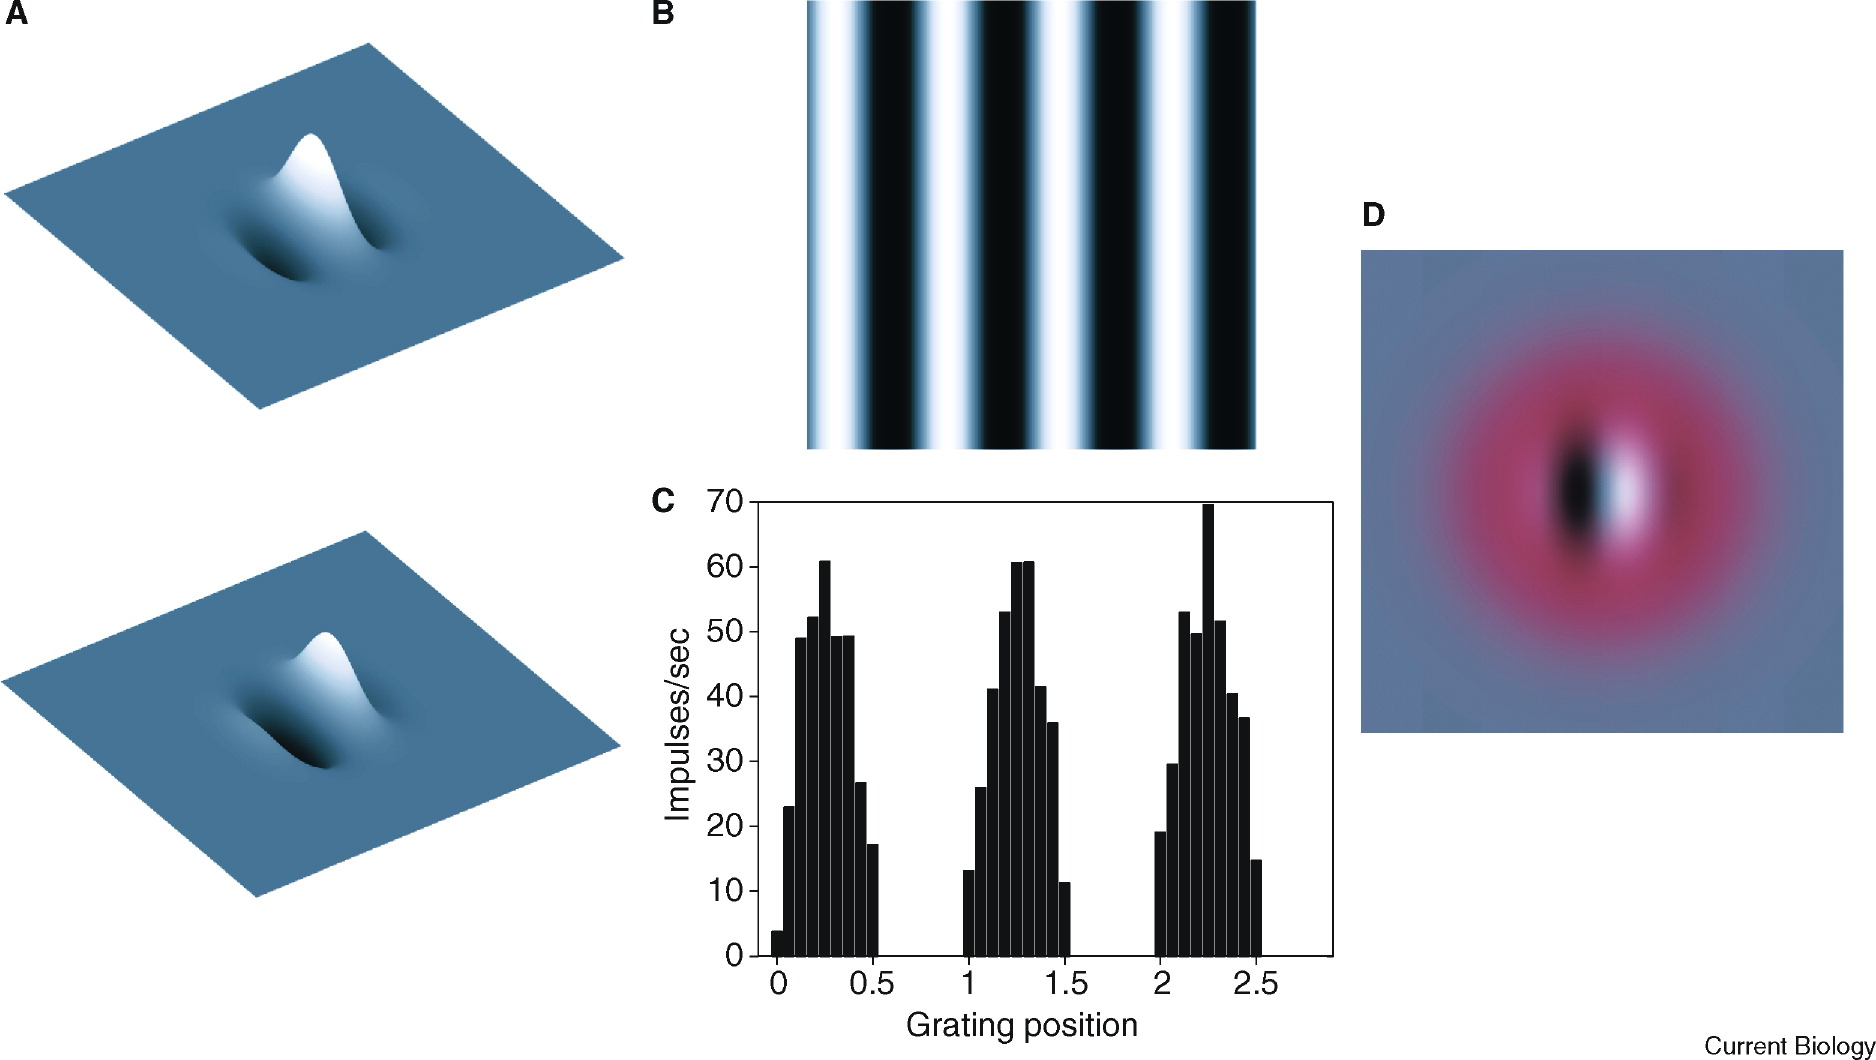
\includegraphics[width=0.5\textwidth]{7-2.jpg}
    \caption{The simple cell RF can be constructed by weighing a sinusoid using two Gaussian filters. \cite{lennie_2003_receptive}}
    \label{fig:6}
\end{figure}


\textbf{A7} Despite rough edges caused by limited subimage resolution, these basis vectors obtained from PCA demonstrate many similarities with receptive fields (RF) of simple cells (Fig~\ref{fig:6}) as they all demonstrate linear filtering properties with clear distinction between inhibitory regions (with negative filter weight) and excitatory regions (with positive filter weight).
However, the inherent linearity of PCA makes accurate representation of non-linear filters of higher-order difficult even with higher complexity. In addition, because the PCs are independent of the phase spectrum of input stimuli \cite{field_1994_what}, the PCA method is also unable to capture local characteristics precisely as a neuron would in V1. \textbf{EOA}

\paragraph{PCA for \textit{I3}}

\textbf{A4} Unlike \textit{I1} and \textit{I2}, PCA on the \textit{I3} random white noise dataset shows no clear trend due to the low correlation between local pixels. However, as seen in Fig~\ref{fig:4}, the filter effectively captures features like immediate intensity contrast. \textbf{EOA}
\begin{figure}[ht]
    \centering
    \subfigure[]{
        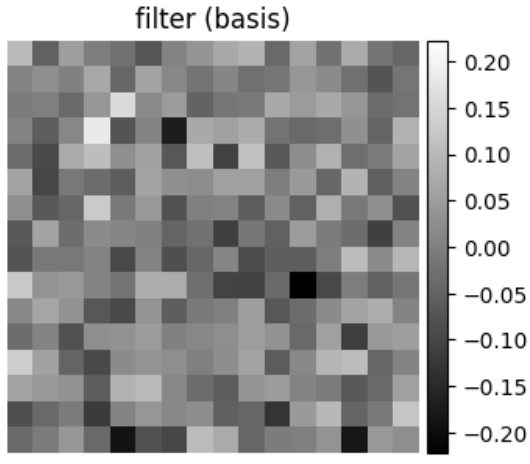
\includegraphics[width=0.155\textwidth]{4-1.png}
    }
    \subfigure[]{
        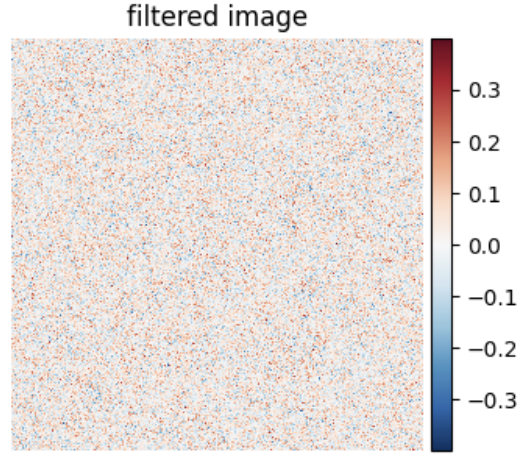
\includegraphics[width=0.16\textwidth]{4-2.png}
    }
    \subfigure[]{
        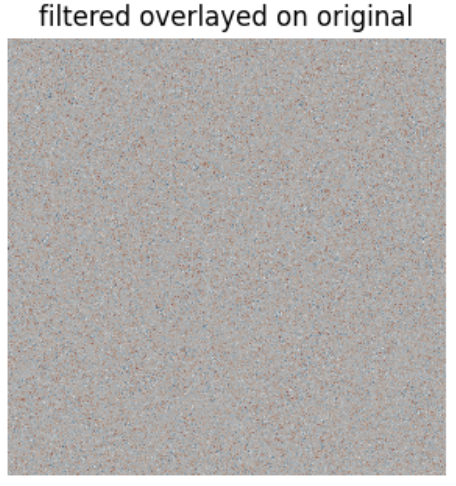
\includegraphics[width=0.13\textwidth]{4-3.png}
    }
    \caption{An example of basis function for random noise \textit{I3}: (a)basis filter, (b)filtered image, (c)filtered image overlayed on original image}
    \label{fig:4}
\end{figure}

\paragraph{Discussion}
Comparing PCA performance across the three datasets, it is evident that compact coding is most effective for images with high local covariance and smaller state spaces, such as natural images, and struggles with randomness. Even for natural images like \textit{I2}, PCA fails to capture certain boundary details processed by V1 neurons, highlighting the need to explore alternative sensory coding strategies, such as sparse coding.

\vspace{-0.5em}

\subsection{Sparse Coding}
\subsubsection{Iterative optimisation}

\vspace{-1em}

In the sparse coding framework, the performance of a code is assessed by the cost function 

\vspace{-2em}

\begin{adjustwidth}{-1.5em}{}
\small
    \begin{equation}
        \label{eq:sparsecost}
        \mathcal{C}\left(\mathbf{B}, \mathbf{A}\right) = \frac{1}{K} \sum_{k=1}^K \left( \sum_j \left[ {S}_{kj} - \sum_i {A}_{ki} \: {B}_{ij} \right]^2
        + \lambda \sum_i \log\left(1+\frac{{A}_{ki}^2}{\sigma^2}\right) \right)
    \end{equation}
\end{adjustwidth}

which is then minimised with respect to both the basis functions $\mathbf{B} = \{{B}_{ij} \}$
and the activations $\mathbf{A} = \{{A}_{ki}\}$. This optimisation is conducted iteratively by first minimising $\frac{\partial \mathcal{C}(\mathbf{A})}{\partial \mathbf{A}}$ for a fixed $\mathbf{B}$, then minimising for $\frac{\partial \mathcal{C}(\mathbf{B})}{\partial \mathbf{B}}$ for the optimum $\mathbf{A}$.

Conveniently writing the expression using the error matrix $\mathbf{E} = \mathbf{S}-\mathbf{AB}$ and trace function, the partial derivatives are found as follows:

\vspace{-2em}

\begin{equation}
    \label{eq:dcda}
    \frac{\partial \mathcal{C}(\mathbf{A})}{\partial \mathbf{A}} = \frac{2}{K} \left( \mathbf{A} \mathbf{B} \mathbf{B}^\top - \mathbf{S} \mathbf{B}^\top \right) + \frac{2 \lambda}{K} \left( \frac{\mathbf{A}}{\sigma^2 + \mathbf{A}^2} \right)
\end{equation}

and \textbf{A8}
\begin{equation}
    \label{eq:dcdb}
    \frac{\partial \mathcal{C}(\mathbf{B})}{\partial \mathbf{B}} = \frac{2}{K} \left(\mathbf{A}^\top \mathbf{A} \mathbf{B} - \mathbf{A}^\top \mathbf{S}\right)
\end{equation}
\textbf{EOA}

\textbf{A9} During the implementation of this optimization algorithm (details in \hyperref[sec:appendix]{Appendix}), $\mathbf{B}$ is normalized at each iteration to improve numerical stability, as it undergoes large updates with a learning rate $\eta = 0.2$. Without normalization, the basis function values in $\mathbf{B}$ could easily explode or vanish due to the unpredictable and potentially large gradient $\frac{\partial \mathcal{C}(\mathbf{B})}{\partial \mathbf{B}}$. \textbf{EOA}

\subsubsection{Interpretation of Bases by Sparse Coding}

\vspace{-0.5em}

Since sparse coding is an infinite iterative process, both the basis functions and their evolution are important. This section compares the sparse coding results for the standard datasets \textit{I2(I2w)} and \textit{I3}, representing extreme cases of natural and artificial images respectively.

\paragraph{Sparse coding basis for \textit{I3}}

\textbf{A10} The basis functions obtained from sparse coding differ significantly from those produced by PCA, as shown in Fig~\ref{fig:10}. Early iterations yield ambiguous receptive fields similar to PCA (Fig~\ref{fig:10-50}), but this resolves as the optimization progresses. By iteration 1000 (Fig~\ref{fig:10-1000}), the receptive fields become sparser and more dispersed, reflecting the goal of sparse coding of promoting overcomplete representations to increase population sparseness and simulate lower action potential requirements for the same neuron activities \cite{olshausen_2004_sparse}.

Observing the trend at different iteration counts, it can be predicted that as number of iteration reaches infinity, each basis function of \textit{I3} will approach a highly simplified filter with only one feature pixel in a background of uniform intensity, which corresponds to zero overall mean (normalised to fill the greyscale).
Therefore, the dataset \textit{I3} could also be reconstructed perfectly by linear superposition and combination of these random filters, given a fully trained set of basis functions. \textbf{EOA}

\begin{figure}[ht]
    \centering
    \subfigure[50 iterations]{
        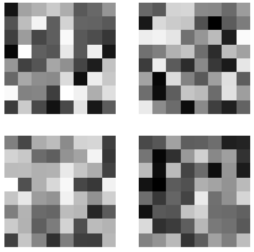
\includegraphics[width=0.23\textwidth]{10-4.png}
        \label{fig:10-50}
    }
    \subfigure[1000 iterations]{
        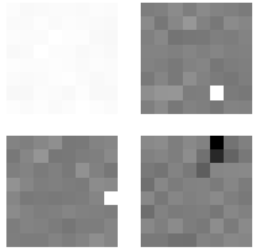
\includegraphics[width=0.23\textwidth]{10-3.png}
        \label{fig:10-1000}
    }
    \caption{An example of a group of four basis functions of \textit{I3} generated by sparse coding, (a)at 50 iterations and (b) at 1000 iterations.}
    \label{fig:10}
\end{figure}

\paragraph{Sparse coding basis for \textit{I2}}

Since \textit{I2} dataset consists of natural images which very different variances along different directions in the $n_{\sf pix}$-dimensional image space, it is pre-processed by whitening to \textit{I2w} as adjacent correlation is removed and variance unified. This whitening process also captures how the retinal ganglion cells decorrelate natural visual stimuli to reduce redundancy and suppress noise for each individual neuron \cite{dodds_2019_spatial}.

\textbf{BA1} In order to implement this batch normalisation method, the PCA-whitening technique is experimented (see details in \hyperref[sec:appendix]{Appendix}). PCA-whitening is a process where the original dataset is multiplied by the matrix of eigenvectors of the covariance matrix, which is then normalised using the square root of its singular values \cite{dodds_2019_spatial}. The covariance matrix is analysed using Singular Value Decomposition (SVD) for the PCA process.
Because the products of this pre-processing step is to be used in training, the full $256 \times 256$ pixels matrix is used for SVD, and a randomly sampled set of subimages is used then to calculate the amount of required scaling for efficiency considerations.

However, as shown in Fig~\ref{fig:b1}, the pre-whitening result from PCA-whitening is not optimum and appears to be not sphericalised enough when comparing to its contemporary in \textit{I2w}. This is conjured to be an effect of the PCA-whitening strategy, which can be modified and likely improved by more complicated algorithms like ZCA. \textbf{EOA}
\begin{figure}[ht]
    \centering
    \subfigure[]{
        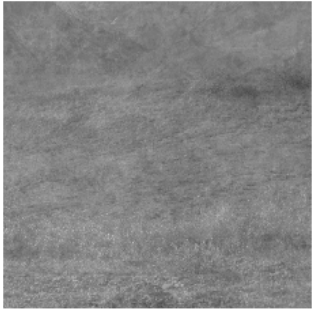
\includegraphics[width=0.23\textwidth]{B1_me.png}
        \label{fig:b1_me}
    }
    \subfigure[]{
        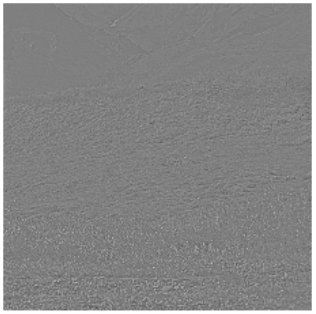
\includegraphics[width=0.23\textwidth]{B1_them.png}
        \label{fig:b1_them}
    }
    \caption{An example of pre-whitened image from \textit{I2}: (a)experimental results from this lab exercise and (b)the corresponding image in dataset \textit{I2w}}
    \label{fig:b1}
\end{figure}

\begin{figure}[ht]
    \centering
    \subfigure[]{
        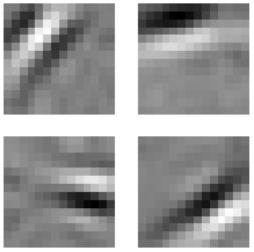
\includegraphics[width=0.23\textwidth]{11-1.png}
        \label{fig:11_me}
    }
    \subfigure[]{
        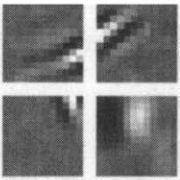
\includegraphics[width=0.23\textwidth]{11-2.png}
        \label{fig:11_of}
    }
    \caption{An example of a group of four basis functions of \textit{I2w} generated by sparse coding. Notice the similarity between (a)experimental results from this lab exercise (3500 iterations) and (b) basis functions learned by sparse coding algorithm in the original paper by Olshausen \& Field \cite{olshausen_1997_sparse}.}
    \label{fig:11}
\end{figure}

\textbf{A11} Although both demonstrate directional discrimination to some extent, it is obvious that the basis functions learned by sparse coding in Fig~\ref{fig:11_me} demonstrates better localisation and clear boundaries for inhibitory and excitatory regions. This also aligns well with the localised and oriented structure of V1 simple cell RF linear filters. \textbf{EOA}

\subsubsection{Measure of Sparseness}
\textbf{BA2} When describing a variable with the term "sparse", two scenarios might be indicated:
\begin{itemize}
    \item Population sparseness: The average number of neurons active at any time,
    \item Lifetime sparseness (kurtosis): Each neuron has a high kurtosis in its lifetime activation responses. \cite{willmore_2001_characterizing}
\end{itemize}

In this lab exercise, since temporal data over a certain time range is unattainable, it is assumed that the sparseness to be measured describes population sparseness. One possible way of measuring this quantity is the "effective PCA" count as discussed in Sec~\ref{sec:dimreduction}.
The kurtosis of response of the entire population to a single visual stimulus could may also be an important indicator, which can be calculated as:
\begin{equation}
    K_P = \left\{ \frac{1}{N} \sum_{j=1}^N \left( \frac{r_j - \bar{r}}{\sigma_r} \right)^4 \right\} - 3  \cite{willmore_2001_characterizing}
\end{equation}
\textbf{EOA}


\section{Conclusion}
In this lab exercise, the performance and characteristics of compact coding and sparse coding are examined as two common strategies for sensory coding. It is observed that compact coding through PCA generates fewer basis functions compared to the overcomplete basis set obtained from sparse coding. However, PCA also falls short in accurately representing the complexity of neuron activity in V1. Sparse coding, on the other hand, provides a more biologically realistic and accurate model of V1 neuron responses by producing sparse, distributed representations, and is hence more suitable for noisy or random stimuli.

These results align with the widely accepted view that sparse coding is a more powerful and efficient strategy for sensory coding, particularly for representing natural images. Nonetheless, PCA remains useful for identifying key features in data through principal components and offers an effective preprocessing method, such as whitening, which reduces redundancy and simplifies subsequent analyses. 
Each with their own strengths and weaknesses, compact and sparse coding are important complimentary tools fostering better understanding of the myths of sensory coding.

\begin{small}
\bibliographystyle{ieeetr}
\bibliography{3G3}
\end{small}

\section*{Appendix: Code implementations}
\begin{appendix}\label{sec:appendix}
\begin{lstlisting}
def cost(A, B, S, lambd, sigma):
"""
cost function

Parameters
----------
A: activations with shape (n_sub, n_bas)
B: bases functions (n_bas, n_pix)
S: matrix of image patches (n_sub, n_pix)
lambd: weighs the importance of reconstruction error and sparsity
sigma: activation scale hyper-parameter in the cost function
    
Returns
-------
c: average cost for the image batch (thus c = err + sparsity; see next two lines)
err: reconstruction error per batch
sparsity: sparsity penalty per batch, including the lambd factor
"""
n_sub = np.shape(A)[0]
    
err = (np.trace(S @ S.T) - 2 * np.trace(S @ B.T @ A.T) + np.trace(A @ B @ B.T @ A.T)) / n_sub

sparsity = lambd * np.sum(np.log(1 + (A ** 2) / (sigma ** 2))) / n_sub

c = err + sparsity

return c, err, sparsity
\end{lstlisting}

\begin{lstlisting}
def dcost_A(A, B, S, lambd, sigma):
"""
gradient of the cost function with respect to A (i.e., dC/dA)

Parameters
----------
A: activations with shape (n_sub, n_bas)
B: bases functions (n_bas, n_pix)
S: image patches (n_sub, n_pix)
lambd: weighs the importance of reconstruction error and sparsity
sigma: activation scale hyper-parameter in the cost function

Returns
-------
dc: gradient of the cost function dC/dA

"""
n_sub = np.shape(A)[0]

dc = (2 / n_sub) * ((A @ B @ B.T) - (S @ B.T)) + (2 * lambd / n_sub) * (A / (sigma**2 + A**2))

return dc
\end{lstlisting}

\begin{lstlisting}
def dcost_B(A, B, S, lambd, sigma):
"""
gradient of the cost function with respect to B (i.e., dL/dB)

Parameters
----------
A: activations with shape (n_sub, n_bas)
B: bases functions (n_bas, n_pix)
S: image patches (n_sub, n_pix)
lambd: weighs the importance of reconstruction error and sparsity
sigma: activation scale hyper-parameter in the cost function

Returns
-------
g: gradient of the cost function dL/dB
"""    
n_sub = np.shape(A)[0]

g = 2 * (A.T @ A @ B - A.T @ S)/ n_sub

return g
\end{lstlisting}

\begin{lstlisting}
    def pca_whiten_image_set(
        images, 
        patch_size=8, 
        n_patches=1000):
"""
PCA-whiten a set of images using statistics from random patches

Parameters
----------
images: numpy.ndarray
Set of images with shape (n_images, n_pixels) e.g. (9, 512*512)
patch_size: int
Size of square patches to extract (default 8)
n_patches: int
Number of random patches to sample (default 1000)

Returns
-------
whitened_images: numpy.ndarray
PCA-whitened images with same shape as input
"""
# Full image SVD to get PCA
_, s, vt = np.linalg.svd(images - np.mean(images, 0), full_matrices=False)

# Sample patches to compute whitening scaling needed while maintaining efficiency
patches = sample_patches(images, patch_size, n_patches)
_, patch_s, _ = np.linalg.svd(patches - np.mean(patches, 0), full_matrices=False)

scaling = np.std(patch_s)

whitened_images = np.zeros_like(images)
for i, img in enumerate(images):
img_centered = img - np.mean(img)
img_proj = img_centered @ vt.T

# Scale the projections using the singular values from patches
whitened_proj = img_proj / (scaling + 1e-5) # Regularisation for numerical safety

whitened_images[i] = whitened_proj @ vt

return whitened_images
\end{lstlisting}


\end{appendix}
\end{document}